\typeout{..... title page}

\makeatletter
% Set tint for Penrose
\tikzset{
tint fill colour/.code={%
\edef\@temp{%
\def\noexpand\tikz@fillcolor{\tikz@fillcolor!#1}%
\noexpand\tikz@addoption{%
\noexpand\pgfsetfillcolor{\tikz@fillcolor!#1}%
}%
}%
\@temp
}
}

% Defining a new coordinate system for the page:
%
% --------------------------
% |(-1,1)    (0,1)    (1,1)|
% |                        |
% |(-1,0)    (0,0)    (1,0)|
% |                        |
% |(-1,-1)   (0,-1)  (1,-1)|
% --------------------------
\def\parsecomma#1,#2\endparsecomma{\def\page@x{#1}\def\page@y{#2}}
\tikzdeclarecoordinatesystem{page}{
    \parsecomma#1\endparsecomma
    \pgfpointanchor{current page}{north east}
    % Save the upper right corner
    \pgf@xc=\pgf@x%
    \pgf@yc=\pgf@y%
    % save the lower left corner
    \pgfpointanchor{current page}{south west}
    \pgf@xb=\pgf@x%
    \pgf@yb=\pgf@y%
    % Transform to the correct placement
    \pgfmathparse{(\pgf@xc-\pgf@xb)/2.*\page@x+(\pgf@xc+\pgf@xb)/2.}
    \expandafter\pgf@x\expandafter=\pgfmathresult pt
    \pgfmathparse{(\pgf@yc-\pgf@yb)/2.*\page@y+(\pgf@yc+\pgf@yb)/2.}
    \expandafter\pgf@y\expandafter=\pgfmathresult pt
}
\makeatother

%%%%%%%%%%%%%%%%%%%%%%%%%%%%%%%%%%%%%%%%%%%%%%%%%%%%%%%%%%%%%%%%%%%%%%%%%%%%
% render the page
\hypersetup{pageanchor=false}
\tikzexternaldisable
\begin{titlingpage}
\begin{tikzpicture}[
overlay, remember picture,nodes={inner sep=0pt,outer sep=0pt},
every Penrose tile/.style={draw=black!70},
every dart/.style={
fill=teal
},
every kite/.style={
fill=orange
},
Penrose tile/.code 2 args={
  \pgfgetlastxy{\cx}{\cy}  
  \path (page cs: -1,-1); \pgfgetlastxy{\ix}{\iy}
  \path (page cs: 1,1); \pgfgetlastxy{\ax}{\ay}
  \pgfmathsetmacro{\ny}{(\cy-\iy)/(\ay-\iy)}
%\pgfmathsetmacro\tint{0.2+80*(#1/#2)}
  \pgfmathsetmacro\tint{0.6*(1.5*#1*#2+30*(2-\ny)+30*random())}
\pgfkeysalso{tint fill colour=\tint}
}
]

\draw[white,fill=teal!15] (page cs:-1,-1) rectangle (page cs:1,1);


\path[save Penrose path=a] (0,0) to[out=-30,in=100] (1,0);
\path[save Penrose path=c] (0,0) to[out=-40,in=140] (1,0);
\BakePenroseTile{kite}
\BakePenroseTile{dart}

\def\tp{kite}
\ifdraftdoc\def\coverLevel{2}\fi

\begin{scope}[shift={(page cs:0,0)}, scale=20]
\foreach[evaluate=\k as \mk using {\k+Mod(\k,2)},evaluate=\k as
\ax using {Mod(\k,2) == 0 ? "T" : "t"}] \k in {0,...,9} {
\begin{scope}[rotate=\mk*36]
\PenroseDecomposition{\tp}{\coverLevel}{\ax}
\end{scope}
}
\end{scope}

\filldraw[fill=teal!10, opacity=0.7, draw=none] (page cs:-1,-0.75) rectangle (page cs:1,-0.25);
\node[anchor = west, right=1.5cm] at (page cs: -1,-0.4){{\fontsize{80pt}{30pt}\yanone PROGRAMOVANIE}};
\node[anchor = east, left=2.1cm] at (page cs: 1,-0.62){{\fontsize{65pt}{30pt}\yanone v C++}};

\end{tikzpicture}
\end{titlingpage}


\begin{titlingpage}
  \epigraph{Cimrman se však nespokojuje jen s kritikou, ale dává příklad vlastními tvůrčími činy. 
  Tady je nutno přiznat, že řada jeho pohádek vzbudila odpor, zejména u dětí.}{{\em --- Divadlo Járy Cimrmana\\ Dlouhý, Široký a Krátkozraký}}

  \vskip 4cm

  \centerline{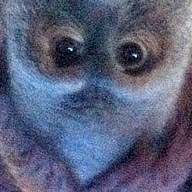
\includegraphics[width=1.5cm]{data/profile.jpg}}
  \vskip 7mm
  \centerline{\begin{minipage}{0.8\textwidth}
  Moje deti sa ma raz spýtali, ako sa programuje. Asi čakali odpoveď na menej ako minútu,
  ja som sa však rozhodol im napísať krátky tutoriál. Krátky tutoriál sa nakoniec trochu 
  rozrástol, zistil som, že to neviem povedať kratšie. Výsledok je tu, poteším sa, ak si ho niekto prečíta. 
    Text aj riešenia úloh sú voľne prístupné
  na Githube na adrese
    \hbox{\href[pdfnewwindow=true]{https://github.com/pocestny/programovanie.git}{https://github.com/pocestny/programovanie.git}}.
  \end{minipage}}
\vfill
v Bratislave \hfill \today
\end{titlingpage}
\hypersetup{pageanchor=true}
\tikzexternalenable

